\documentclass[pdf,xcolor=svgnames]{beamer}

\usepackage[utf8]{inputenc}
\usepackage{graphicx}
\usepackage{helvet}
\usepackage{hyperref}
%\usepackage{listings}


\usetheme{Hannover}
\usecolortheme[named=FireBrick]{structure} 
\setbeamercovered{transparent}


\title[d3lp0r]{\texttt{d3lp0r:}\\\large{A team for the Multi-Agent Programming Contest, based on argumentative BDI agents}}
\author{LIDIA}
\institute{Universidad Nacional del Sur} %\\\email{\{igarai,diegomarcov,leos.molas,%
% emm.montenegro,fsisul,jmtorresluc\}@gmail.com,\\\{sg,ajg,dcm,grs\}%
% @cs.uns.edu.ar}}

\date{November 11, 2011}

\begin{document}

% outline 
% \AtBeginSection[]
% {
 % \begin{frame}
  % \frametitle{Secciones}
  % \small
  % \tableofcontents[currentsection,hideothersubsections]
  % \normalsize
 % \end{frame}
% }

%%%%%%%% FRAME %%%%%%%%%%%%

\begin{frame}
\titlepage

\end{frame}


%%%%%%%% FRAME %%%%%%%%%%%%

\section{Introduction}

\begin{frame}
\frametitle{Introduction}
\begin{block}{}
In the context of the Multi-Agent Programming Contest 2011, organized by the Clausthal University of
 Technology, we developed a multi-agent system. It's based on the BDI architecture, and uses \textbf{Argumentation} (via Defeasible Logic Programming) in the decision making process.
\end{block}
\end{frame}

%%%%%%%% FRAME %%%%%%%%%%%%

\section{Scenario}

\begin{frame}

\frametitle{The scenario}

\begin{block}{Story}
In the year 2033, humans are surviving in the surface of \textbf{Mars}. They 
depend of their robots to gather water supplies. Sadly, this results in sabotage among different groups of settlers.
\end{block}
\pause

The surface of Mars is represented with an \textbf{undirected graph}, in which 
nodes are valid agent locations weighted by value, and edges are valid
transitions weighted by cost. 
\pause

The goal is to maximize the score function each step. A team is awarded
points according to the value of the nodes controlled by the team, and
in addition certain \textit{achievements}.
\end{frame}

%%%%%%%% FRAME %%%%%%%%%%%%

\begin{frame}
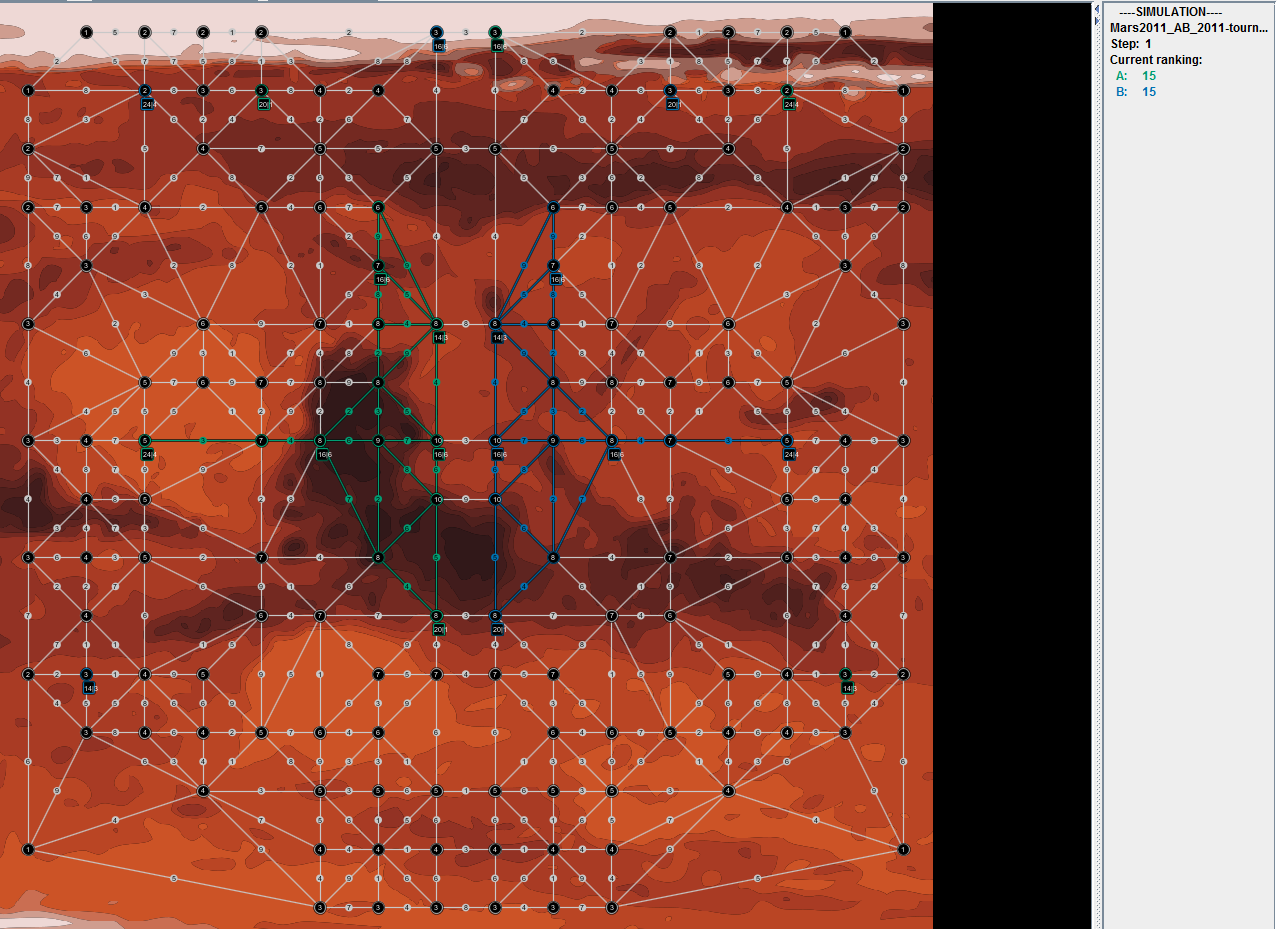
\includegraphics[width=\textwidth]{monitor.png}
\end{frame}

%%%%%%%% FRAME %%%%%%%%%%%%

\begin{frame}
\frametitle{Agent roles}
Agent state includes energy, health, and strength parameters. Agent percepts
include visible nodes, edges, and other agents. 
Each agent is assigned a role in the simulation:

\pause
\begin{itemize}
\item Explorer
\item Repairer
\item Sentinel 
\item Saboteur
\item Inspector
\end{itemize} 
\pause

They determine their valid actions and
initial maximum values for the agent state parameters. 

\end{frame}

%%%%%%%% FRAME %%%%%%%%%%%%

\section{Design}

\begin{frame}
\frametitle{Our approach}
The solution follows a decentralised architecture in which agents run 
completely decoupled in different processes while sharing nothing. Percepts 
are communicated among agent members of the team via a broadcast mechanism 
developed as part of the multi-agent system. This design was chosen for its 
minimal complexity.
\end{frame}

%%%%%%%% FRAME %%%%%%%%%%%%

\begin{frame}
\center
 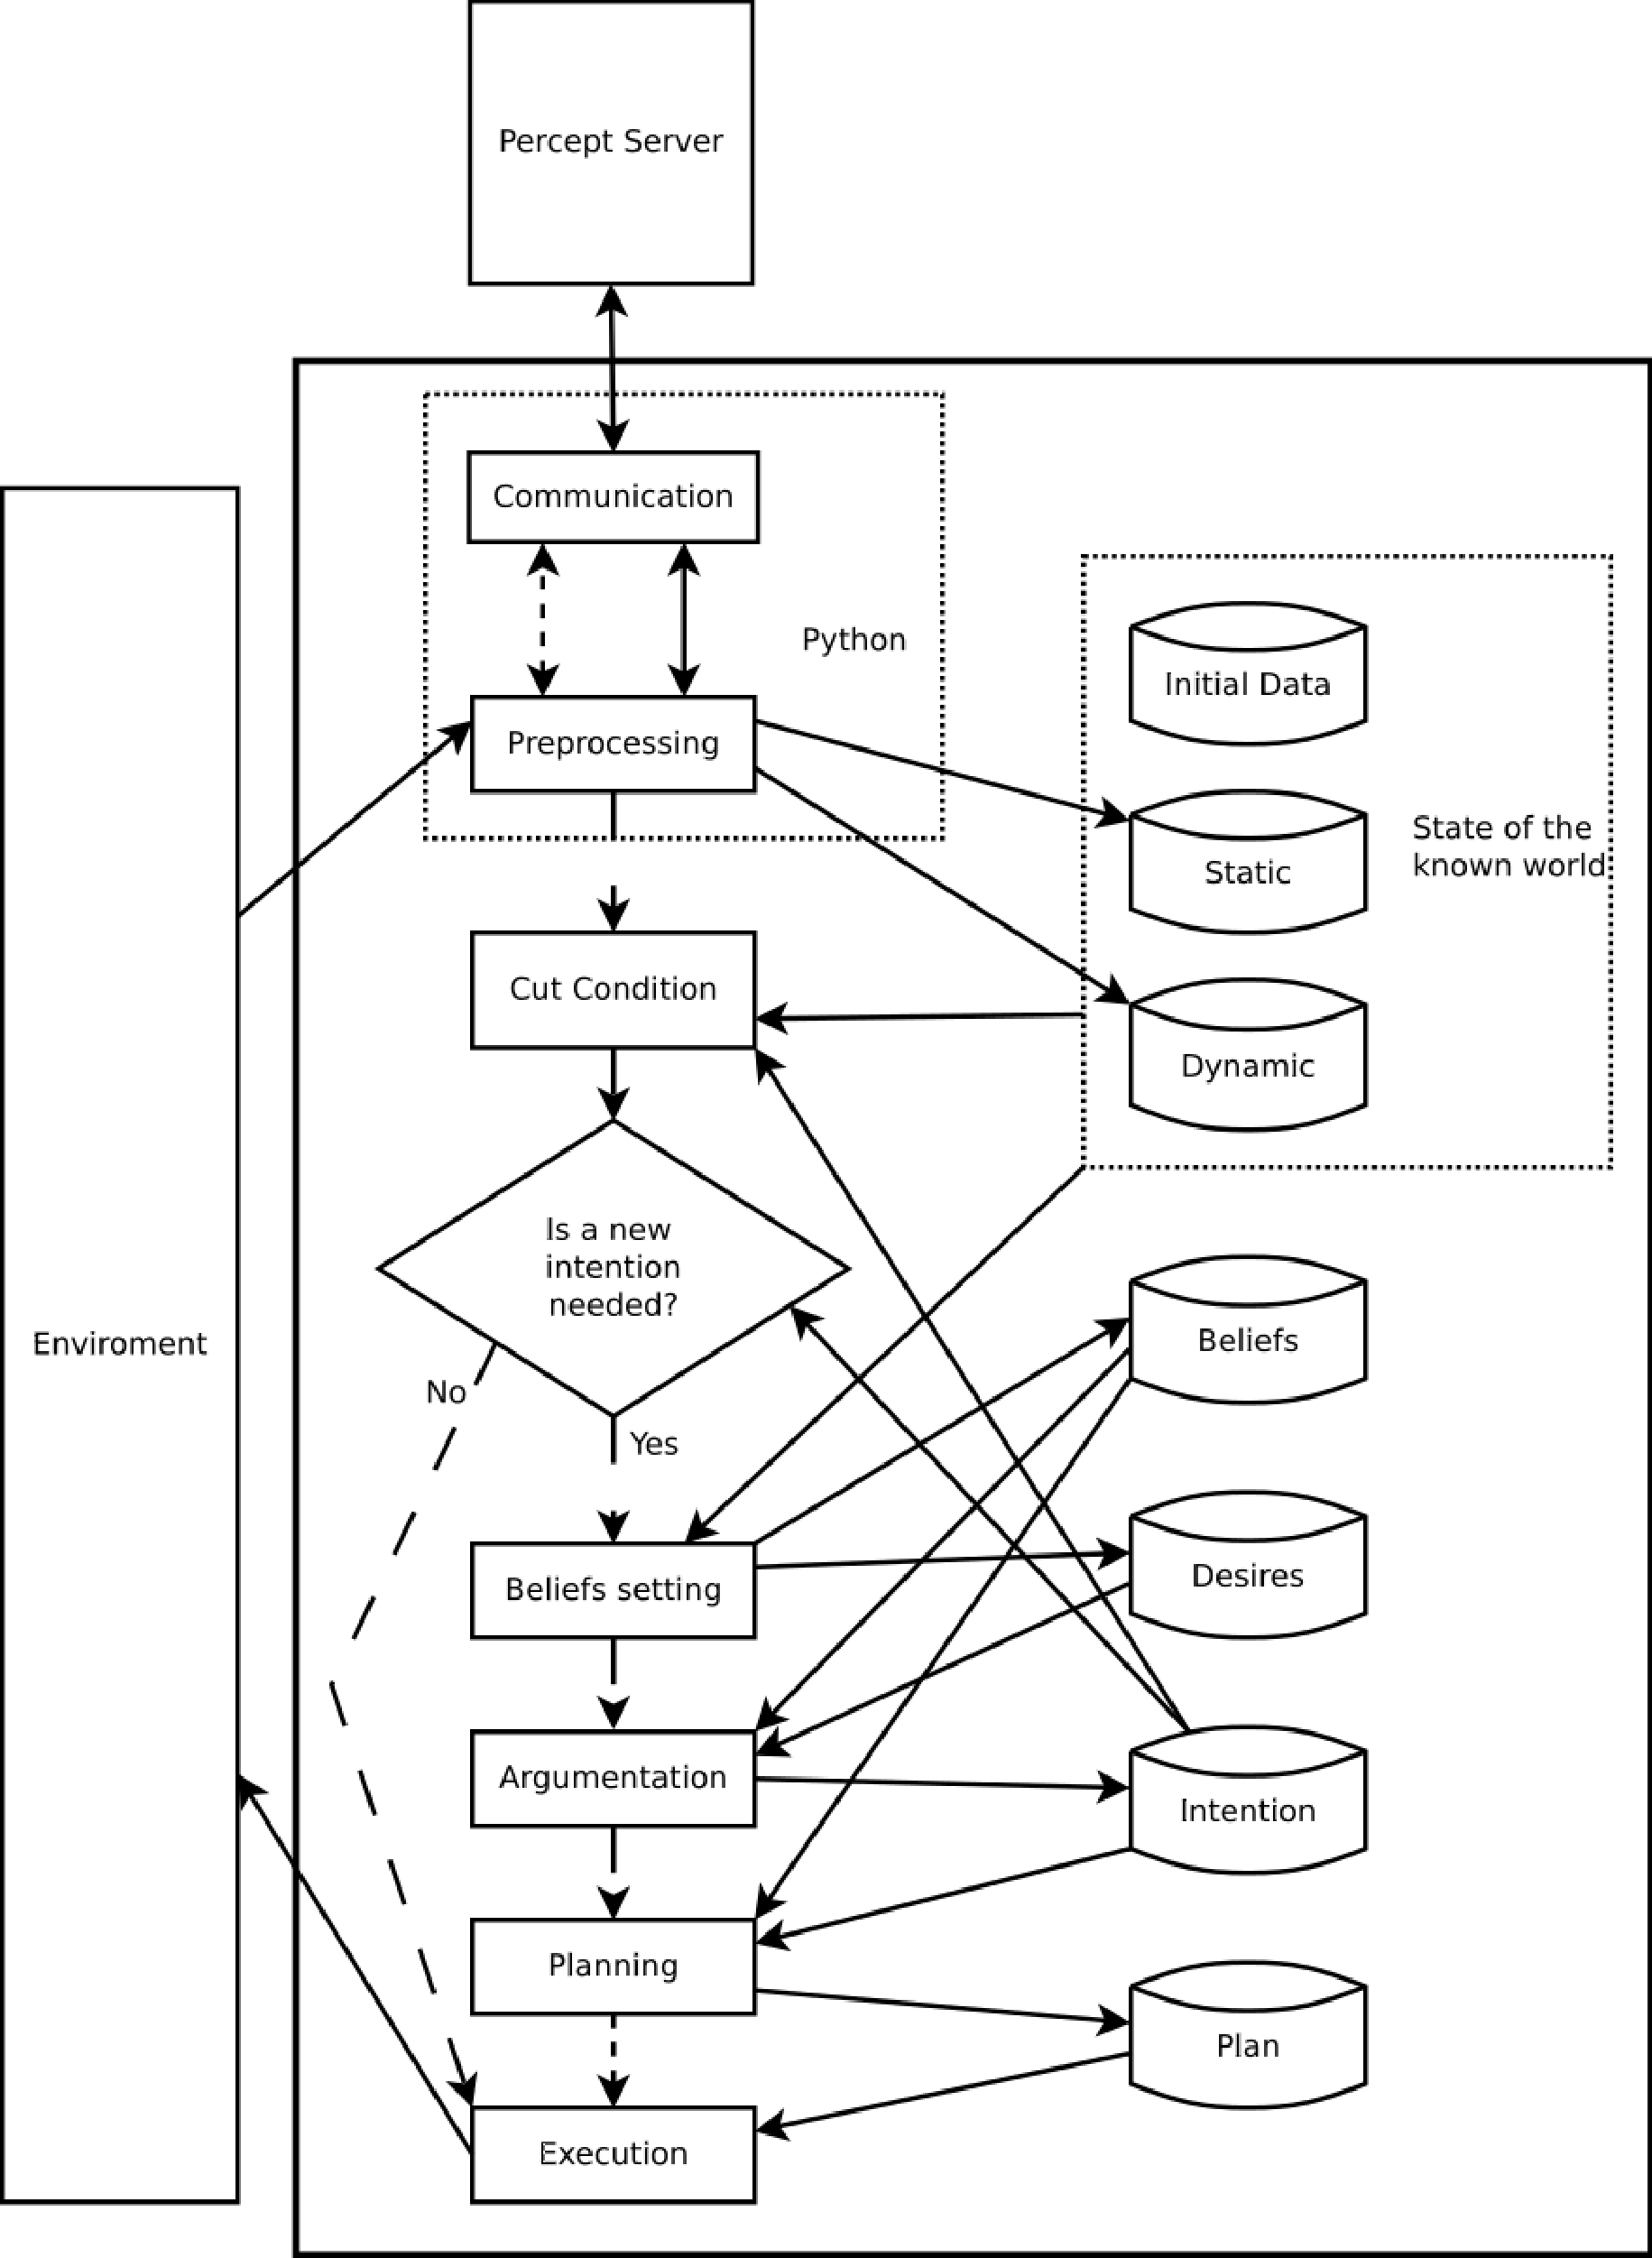
\includegraphics[height=\textheight]{agent_architecture.pdf}

\end{frame}

%%%%%%%% FRAME %%%%%%%%%%%%

\begin{frame}
\center
 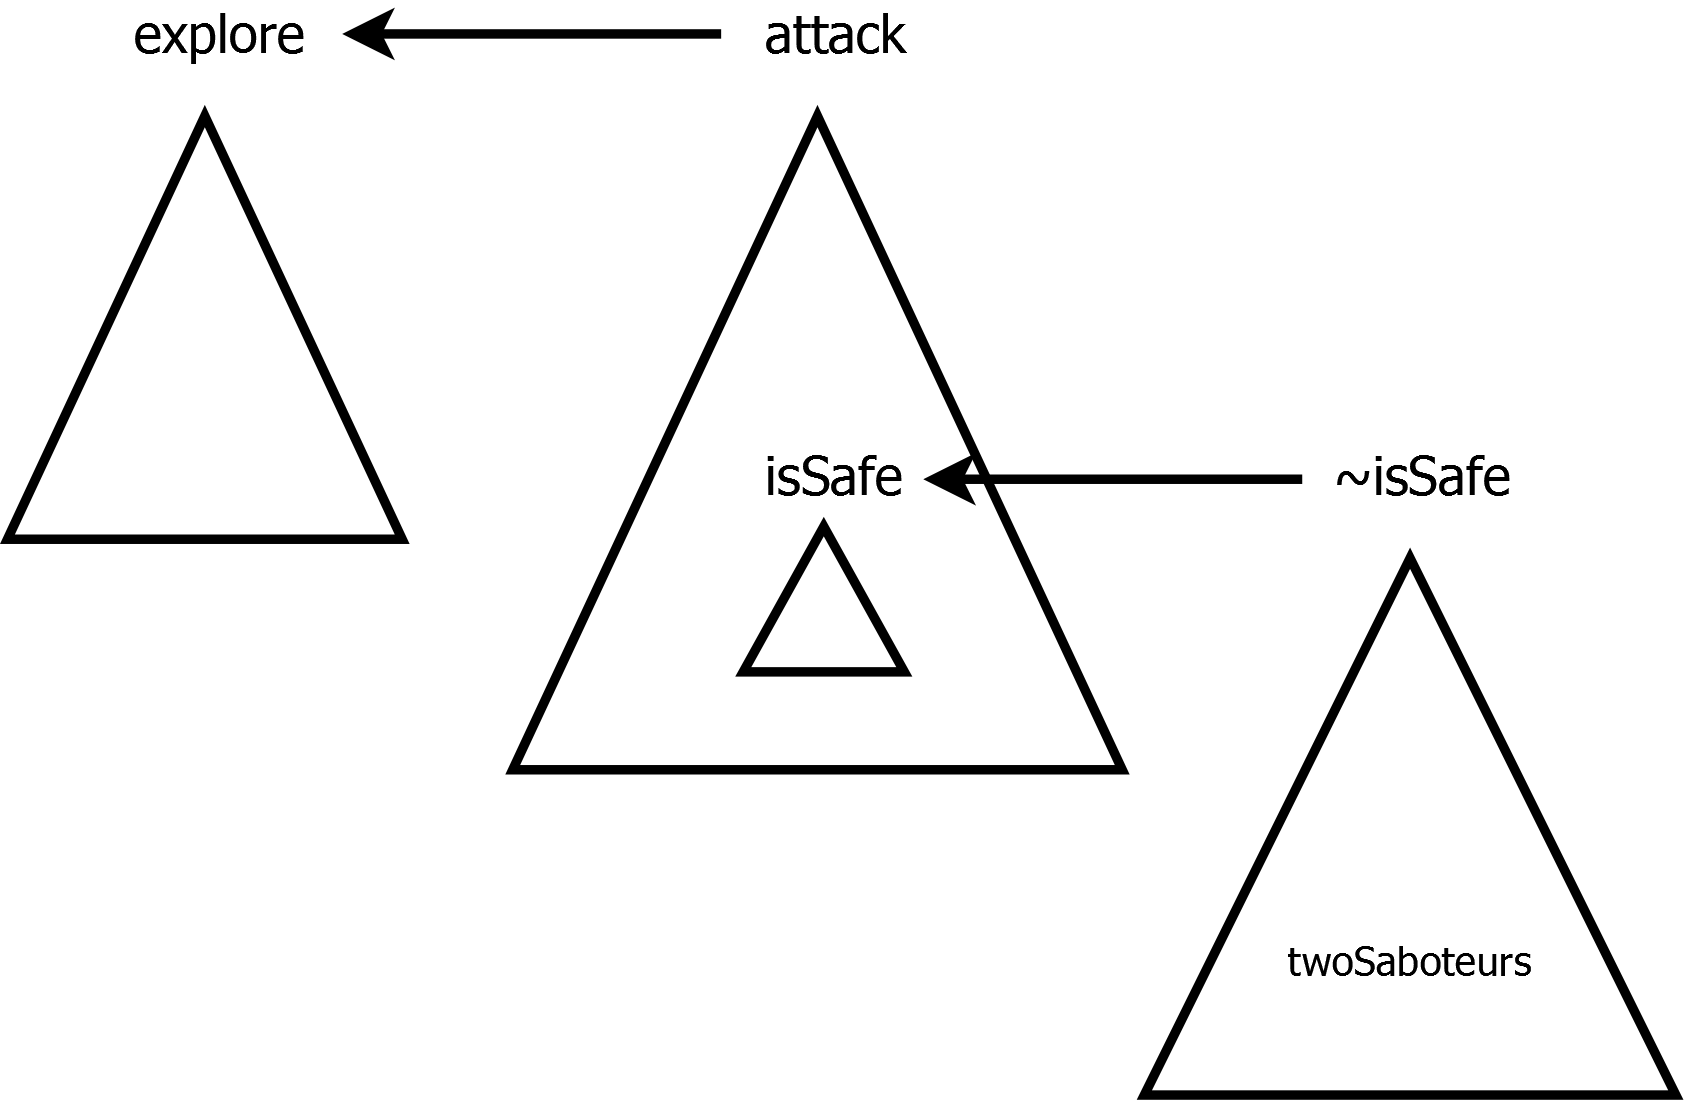
\includegraphics[width=\textwidth]{mamarracho.png}

\end{frame}

%%%%%%%% FRAME %%%%%%%%%%%%

\begin{frame}[fragile]
% aumento(Value, X) -<
    % b(distancia(X, [], Dist, EnergyLeft)),
    % esSeguro(X),
    % b(difPuntosZona(X, DifPuntos)),
    % greater(DifPuntos, 0),
    % phaseCoef(aumento, Coef),
    % aumentoValue(Dist,  DifPuntos, EnergyLeft, 
        % Coef, Value).

\begin{verbatim}
expansion(Value, Node) -<
    distance(Node, Distance),
    zoneDifference(Node, Difference),
    isSafe(Node),
    expansionValue(Distance, Difference, Value).
    
~isSafe(Node) <-
    twoSaboteurs(Node).
    
~expansion(_Value, Node) <-
    zoneDifference(Node, Difference),
    lessOrEqual(Difference, 0).
        
\end{verbatim}
\end{frame}

\end{document}